\chapter*{\textbf{Эксперимент №4: Исследование способов эффективного чтения оперативной памяти}}
\addcontentsline{toc}{chapter}{Эксперимент №4: Исследование способов эффективного чтения оперативной памяти}

\subsection*{\textbf{Цель эксперимента}}
Исследование возможности ускорения вычислений благодаря использованию структур данных, оптимизирующих механизм чтения оперативной памяти.

\subsection*{\textbf{Исходные данные}}
Адресное расстояние между банками памяти, размер буфера чтения.

\subsection*{\textbf{Описание проблемы}}
При обработке информации, находящейся в нескольких страницах и банках оперативной памяти возникают задержки, связанные с необходимостью открытия и закрытия страниц DRAM памяти. При программировании на языках высокого уровня такая ситуация наблюдается при интенсивной обработке нескольких массивов данных или обработке многомерных массивов. При этом процессоры, в которых реализованы механизмы аппаратной предвыборки, часто не могут организовать эффективную загрузку данных. Кроме этого, объемы запрошенных данных оказываются заметно меньше размера пакета, передаваемого из оперативной памяти. Таким образом, эффективная обработка нескольких векторных структур данных без их дополнительной оптимизации не использует в должной степени возможности аппаратных ресурсов. 

\subsection*{\textbf{Результаты эксперимента}}
На рисунке \ref{img:experiment_4} представлен график, полученный в результате эксперимента с исходными параметрами:
\begin{itemize}
	\item Размер массива (М) = 2;
	\item Количество потоков данных = 64.
\end{itemize}

\begin{figure}[H]
	\centering{
		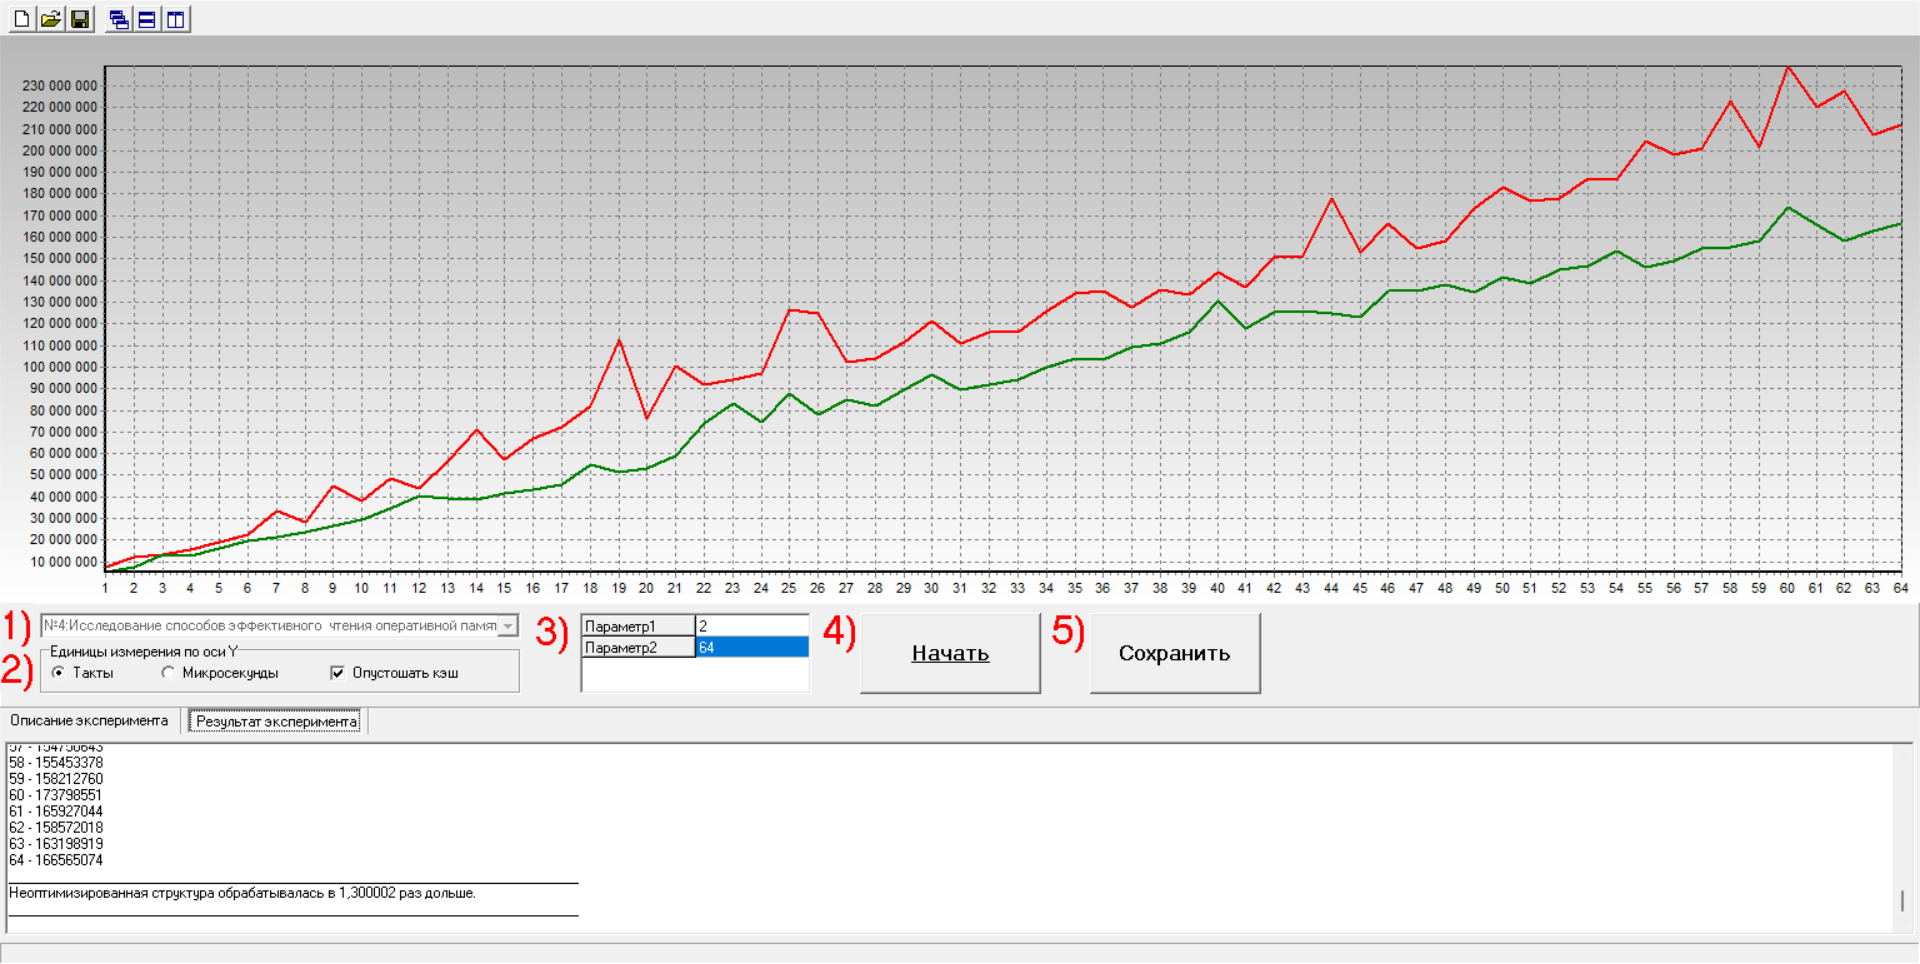
\includegraphics[scale=0.4]{images/experiment_4_1}
		\caption{Эксперимент №4}
		\label{img:experiment_4}
	}
\end{figure}

Результат сравнения времени (как вывод программы) представлен на рисунке \ref{img:experiment_4}. Как видно на рисунке, неоптимизированная структура обрабатывалась в 1,30 раз дольше.

Красный график показывает время или количество тактов работы алгоритма, использующего неоптимизированную структуру.

Зеленый график показывает время (или количество тактов) работы алгоритма с использованием оптимизированной структуры.

Оптимизация заключается в том, что структура данных, ускоряющая обработку современным процессорам, пытается максимально исключить несвоевременную передачу данных, то есть передавать только лишь востребованную для вычислений информацию. Поэтому снижается количество открытий и закрытий страниц DRAM-памяти и обеспечивается параллельная обработка данных, а также выполнение операций загрузки и выгрузки.


\subsection*{Вывод}
Для ускорения работы алгоритмов, необходимо правильно упорядочить данные.